\chapter{State of the Art} \label{chap:sota} \minitoc

In this Chapter, we discuss the most relevant work for the aforementioned problem of detecting data pattern shifts in real-time computations over true sliding windows using resource-lightweight approaches on streaming systems. We present a wide analysis of several categories of algorithms that seemed like viable options to build the desired system.

\section{Data Mining} \label{sec:change-detect}
A data stream has a temporal dimension and the underlying process that generates the data stream can change over time \cite{Aggarwal-Evolving-Data-Streams} \cite{Domingos-Mining-Time-Data-Streams}. It is this change in the underlying distribution that we want to detect and report as a data pattern shift.

\subsection{A two window paradigm algorithm for change detection}
\label{subsec:2-window}

Kifer et al. propose an algorithm for change detection in data streams \cite{Kifer-Detecting-Change}. The authors propose that detecting change in data streams can be reduced to testing if two windows have different underlying distributions. Thus the change detection algorithm works on a two-window paradigm.

Figure \ref{fig:change-detection-2-windows} contains the pseudocode presented by the authors. The proposed method uses two windows, a reference \textit{W\textsubscript{1}} and a sliding one \textit{W\textsubscript{2}}. The authors use tuple-based windows of size \textit{k} and a true sliding window. The reference window \textit{W\textsubscript{2}} works as a \textit{baseline} and contains the first \textit{k} points of the stream that occurred after the last detected change.

The algorithm begins by filling both windows with the first \textit{k} tuples. Then it slides window \textit{W\textsubscript{2}} (by one tuple, since it is a true sliding window). It does this \textit{k} times and in between slides checks for change by applying the \textit{d} function, which measures the discrepancy between the two windows, \textit{W\textsubscript{1}} and \textit{W\textsubscript{2}}. Whenever this discrepancy is above a certain threshold $\alpha$, the algorithm reports a change in the data stream. Then it repeats the whole process, re-initializing both windows with the next \textit{k} items and proceeding as already described. 

\begin{figure}[!htb]
    \begin{center}
      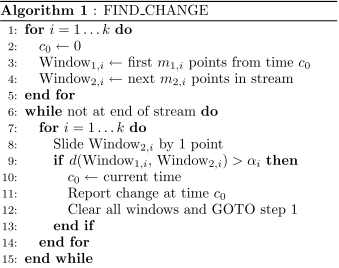
\includegraphics[scale=0.8]{figures/2-windows-change-pseudocode.png}
      \caption{Two window method for data stream change detection}
      \label{fig:change-detection-2-windows}
    \end{center}
\end{figure}

This algorithm reduces change detection in data streams to testing whether two samples --- \textit{reference} and \textit{sliding} windows --- are generated by different distributions. The authors study methods for identifying differences in distribution between two samples and implement them as the \textit{d} function. Furthermore, they develop their own data structure and algorithm for efficient computation of \textit{d}.

%init - \textit{O(klog(k))}    
%runtime - \textit{O(klog(k)}

%k to initialize and when change is detected
%k * d
%d 
 %nlog(2k) to initialize tree and when change is detected
 %log(2k) to maintain the tree
\subsubsection*{Time complexity analysis}
Computing the value of \textit{d} can be done in \textit{O(log(k))} time per iteration. Hence, given \textit{k} iterations, the time complexity of this algorithm is \textit{O(k log(k))}.

\subsubsection*{Space complexity analysis}
The presented algorithm makes use of two \textit{k} sized windows and a custom data structure used for the efficient computation of \textit{d} of size \textit{k} as well. Since \textit{k} is constant, this method has constant space complexity.

\subsubsection*{Applicability to our Hypothesis}
In this Thesis, we want to detect and alert data pattern shifts so detecting change in data streams is directly applicable to our use case. However, our focus is on a lightweight solution and this algorithm has a linear space complexity, so it does not fit our scope as a possible solution.

%\subsection{Pattern Mining}

\subsection{Mining Frequent Patterns: the FP-Stream structure}
An alternative approach to detecting changes in data streams is to perform pattern mining. The idea behind using pattern mining algorithms being that if we can maintain a list of frequent patterns we would be able to detect when said patterns change --- \textit{i.e.} the list changes. Changes in the frequent mined patterns would be associated with a data pattern shift and immediately reported. 

The authors of \cite{Giannella-Mining-Frequent-Patterns} developed a data structure named \textit{FP-Stream} --- that summarizes frequent data patterns -- and algorithms to build and incrementally maintain it.

We agree with the author's statement that it is \textit{"unrealistic to hold all streaming data in the limited main memory"}. With this in mind, they divide patterns into three categories: frequent, sub-frequent and infrequent patterns. The focus of their work is the mining and maintenance of frequent and sub-frequent patterns since the latter might become frequent later. Thus, infrequent patterns are discarded, using less memory.

The FP-Stream structure consists of a frequent pattern tree (FP-Tree \cite{Han-FP-tree}) with tilted-time windows in each of the nodes.

The authors are not very explicit on the definition of a tilted-time window. They claim we are \textit{"often interested in recent changes at a fine granularity, but long term changes at a coarse granularity"} and that tilted-time windows fit such use case. Figure \ref{fig:tilted-time-window} shows such a window and was withdrawn from the paper. In it, we see the 4 quarters of the last hour, then the last 24 hours and finally 31 days. They claim that \textit{"one can compute frequent itemsets in the last hour with the precision of quarter of an hour, the last day with the precision of hour, and so on, until the whole month"}.


\begin{figure}[!htb]
    \begin{center}
      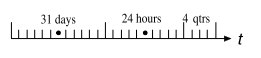
\includegraphics[scale=1]{figures/tilted-time-window.png}
      \caption{Tilted-time window}
      \label{fig:tilted-time-window}
    \end{center}
\end{figure}

An FP-Tree \cite{Han-FP-tree} as shown in Figure \ref{fig:fptree}, is a tree representation of frequent patterns. Each node in the frequent pattern tree represents a pattern and its frequency (\textit{support} column in the Figure), recorded in the node. The same tree construction algorithm from \cite{Han-FP-tree} is used in the FP-Stream algorithm. 

\begin{figure}[!htb]
    \begin{center}
      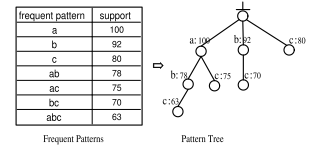
\includegraphics[scale=1]{figures/fptree.png}
      \caption{FP-Tree}
      \label{fig:fptree}
    \end{center}
\end{figure}

The authors propose using only one frequent pattern tree, where at each node, the frequency for each tilted-time window is maintained. Figure \ref{fig:fpstream} shows the FP-Stream structure, as an example of a frequent pattern tree with tilted-time windows embedded in each node.

\begin{figure}[!htb]
    \begin{center}
      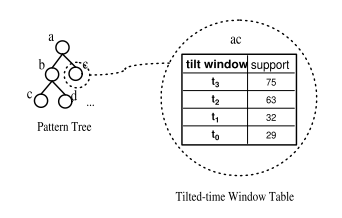
\includegraphics[scale=0.8]{figures/fp-stream.png}
      \caption{FP-Stream}
      \label{fig:fpstream}
    \end{center}
\end{figure}

The algorithm for constructing and maintaining the FP-Stream structure is given as a high-level list of instructions. The algorithm groups incoming streaming data into batches. Initialization is done only when the first batch is complete. As the transactions for the first batch arrived, the frequencies for all items are computed. Once all transactions for the first batch have arrived, the batch is scanned to create an FP-tree structure, pruning all infrequent items -- \textit{i.e.} below a certain frequency threshold. Finally, an FP-Stream structure is created by mining the frequent items from the FP-Tree.

The incremental update of the FP-Stream as data arrives is described on a very high level and does not add relevant information to understand time and space complexity without knowledge of the FP-Tree algorithm, on which it heavily relies. Further research will be done to perform a more thorough analysis of this algorithm, starting with the analysis of \cite{Han-FP-tree}.

\subsubsection*{Applicability to our Hypothesis}

No definitive conclusions can be made without the full time and space complexity analysis. However, the maintenance of a frequent pattern tree and tilted-time windows for each of the nodes might reveal to memory intensive, discarding this as a valid solution.

\subsection{Neighbor-Based Pattern Detection for Windows Over Streaming Data: the Extra-N algorithm}

The authors of \cite{Yang-Neighbor-Based-Pattern-Detection} propose a method for incremental detection of neighbor based patterns, namely density-based clusters and distance-based outliers, specifically for sliding windows scenarios. Figure \ref{fig:plot-cluster-outlier} is an example of the previous two mentioned neighbor based patterns. Formal definitions for both distance-based outliers \ref{fig:distance-outlier-def} and density-based clusters \ref{fig:density-cluster-def} are provided.

\begin{figure}[!htb]
    \begin{center}
      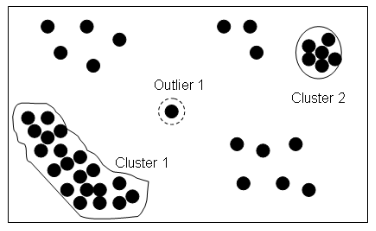
\includegraphics[scale=0.8]{figures/density-distance-based.png}
      \caption[Clustering and outlier identification plot]{Two density-based clusters and one distance-based outlier determined by neighbour-based pattern detection algorithms}
      \label{fig:plot-cluster-outlier}
    \end{center}
\end{figure}

\begin{figure}[!htb]
    \begin{center}
      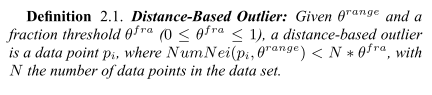
\includegraphics[scale=0.8]{figures/distance-based-outlier-def.png}
      \caption{Formal definition of distance-based outliers}
      \label{fig:distance-outlier-def}
    \end{center}
\end{figure}

\begin{figure}[!htb]
    \begin{center}
      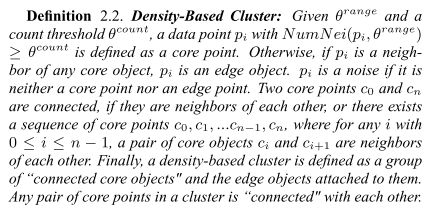
\includegraphics[scale=0.8]{figures/density-based-cluster-def.png}
      \caption{Formal definition of density-based clusters}
      \label{fig:density-cluster-def}
    \end{center}
\end{figure}

Density-based clusters label data points as \textit{core points}, \textit{edge points} or \textit{noise}. These classifications are explained in \ref{fig:density-cluster-def}. Data points are classified based on the number of neighbors they have within a range $\theta\textsuperscript{range}$, measured versus a $\theta\textsuperscript{count}$. In brief, if a data point has more than $\theta\textsuperscript{count}$ neighbors within $\theta\textsuperscript{range}$ it is classified as a \textit{core point}. If it does not but it is a neighbor of a core point, then it is an \textit{edge point}. Otherwise, it is considered \textit{noise}. 

The authors make use of the \textit{“predictability"} property of the expiration of existing objects. In other words, given a window with a fixed slide size, they predetermine the \textit{life-span} of any data point in the window on arrival --- \textit{i.e.} the future windows it will belong to. This leads to the notion of \textit{predicted views}. Given the objects in a current window, they predict the pattern structures that will persist in subsequent windows by considering the objects in the current window and abstract these predicted pattern structures into \textit{“predicted views"} of each future window. This technique allows the efficient maintenance of neighborship counts by pre-handling the eventual expiring effect of new data points.

In the paper, the authors first propose the Abstract-C and Abstract-M algorithms. Ultimately, they combine all the desirable properties of each algorithm into Extra-N. 

\subsubsection{Abstract-C}
Abstract-C was the first proposed algorithm. The main idea is to maintain for each data point \textit{p\textsubscript{i}} the number of neighbors it has rather than the actual list of neighbors. The main advantage of this approach is the reduced memory footprint since only a count is stored --- a single integer --- instead of a list of pointers --- to all neighbors.

When a data point \textit{p\textsubscript{i}} expires, the count of each of \textit{p\textsubscript{i}}'s neighbors must be decremented by one --- since \textit{p\textsubscript{i}} no longer exists. However, we are unable to reach \textit{p\textsubscript{i}}'s neighbors since in Abstract-C only a count of neighbors is stored --- rather than pointers to each of the neighbors.

The solution to this problem is exploiting the previously presented \textit{predictability} property. The key idea is to predict the expiration of any data point \textit{p\textsubscript{i}} and pre-handle the impact it has on \textit{p\textsubscript{i}}'s neighbours. The authors introduce the concept of \textit{"lifetime neighbour counts"} or \textit{lt\_cnt}. The \textit{lt\_cnt} of a data point \textit{p\textsubscript{i}} corresponds to a sequence of \textit{predicted neighbour counts} --- \textit{i.e.} the number of \textit{predicted neighbours} \textit{p\textsubscript{i}} has in any future window where he exists. More precisely, each entry on \textit{pi.lt\_cnt} records the number of \textit{p\textsubscript{i}}'s current neighbours that are known to survive in the corresponding future window. Furthermore, the length of \textit{p\textsubscript{i}.lt\_cnt} is kept equal to \textit{p\textsubscript{i}.lifespan}, decreasing by one after each window slide, removing the left most entry. The authors provide the following example: consider a window \textit{W\textsubscript{i}} and a data point \textit{p\textsubscript{i}} with three neighbours, \textit{p\textsubscript{1}}, \textit{p\textsubscript{2}} and \textit{p\textsubscript{3}}. Applying the \textit{predictability} property makes it possible to compute the lifespan of all points. Assume \textit{p\textsubscript{1}} expires after \textit{W\textsubscript{i}}, \textit{p\textsubscript{2}} and \textit{p\textsubscript{3}} expire after \textit{W\textsubscript{i+1}} and \textit{p\textsubscript{i}} expires after \textit{W\textsubscript{i+2}}. This implies that at \textit{W\textsubscript{i}}, \textit{p\textsubscript{i}.lt\_cnt} = \{\textit{W\textsubscript{i}}: 3, \textit{W\textsubscript{i+1}}: 2, \textit{W\textsubscript{i+2}}: 0\}. 

According to the definition given in \ref{fig:distance-outlier-def}, the lifetime neighbor counts (\textit{lt\_cnt}) carry enough information to compute distance-based outliers: for each data point \textit{p\textsubscript{i}} check if the first (current) element of \textit{p\textsubscript{i}.lt\_cnt} is less than  \textit{$\theta\textsuperscript{fra}$} $\times$ \textit{N} to decide whether a data point is an outlier or not, with \textit{N} as the number of data points. Similarly, the core objects for the density-based clusters can be computed by comparing the first element of \textit{p\textsubscript{i}.lt\_cnt} with \textit{$\theta$\textsuperscript{count}}. However, the \textit{lt\_cnt} array does not carry enough information to generate the density-based clusters. Despite being able  to find all core points in the window, we can not group them into clusters. In order to compute that, Abstract-C analyzes each core point and the surrounding $\theta\textsuperscript{range}$ area in the window to reconstruct the clusters.

In conclusion, Abstract-C achieves linear memory consumption in the number of data points in the window. However, since it reconstructs the clusters for each core object in the window, it has \textit{O(CP)} time complexity, with \textit{CP} as the total number of core points. Hence, its performance largely depends on  \textit{CP}, which can vary from 0 -- no core points --- to the total window size --- all core points. 

\subsubsection{Abstract-M}
Abstract-M is proposed as an Abstract-C enhancement by introducing the notion of \textit{cluster memberships}, achieved by attributing a \textit{clusterID} to each data point.

The main challenge of this approach is discounting the effect of expired data points. The removal of any data point on any cluster may result in the total break of the cluster into multiple smaller ones, which may persist or degrade to noise. Furthermore, when a cluster is split, the newly formed clusters must be attributed with new \textit{clusterID}s --- \textit{i.e.} every single data point in those clusters must be relabeled with the new \textit{clusterID}.

Once again, the solution to handle expiring data points relies on the predictability property. Knowing the data points that exist in each window means we can also know the set of future clusters and points that belong. This is included in the \textit{predicted views} concept previously mentioned. In brief, the \textit{predicted clusters} are created using such predicted views for each of the future windows.

Addition of new data points may cause three changes to the clusters: \textit{birth} of a new cluster, \textit{expansion} of an existing one and \textit{merge} of multiple existing clusters. When adding a new data point, mark it with a new \textit{clusterID} in case of a \textit{birth} or in an \textit{expansion} case mark it with the \textit{clusterID} of the cluster it belongs to. Handling the \textit{merge} of multiple clusters is done by using a tree structure where two or more sibling \textit{clusterID}s are in fact part of a bigger cluster with the \textit{clusterID} stored in their parent. For example, if cluster \textit{ID1} and cluster \textit{ID2} are merged into a new cluster \textit{ID3} by the arrival of a new data point, they are inserted as children of the node containing \textit{ID3}.

New data points may join existing neighborhoods of existing data points and may promote them to core points by making the size of their neighborhood greater or equal to \textit{$\theta$\textsuperscript{count}}. Once such promotion happens, the promoted core point needs to communicate to its neighbors its new role, since noise in its neighborhood becomes edge points and is given a \textit{clusterID}. Since there are no connections from the promoted data point to its neighbors, Abstract-M analyzes each of the promoted core points and the $\theta\textsuperscript{range}$ area around them to find the points requiring state update. 

In conclusion, Abstract-M remains linear in memory regarding the number of window data points. However, since the number of promoted core points tends to be smaller and is always less or equal to the number of core points, this is an improvement on Abstract-C.

\subsubsection{Extra-N}

Abstract-M still performs range queries (area with $\theta\textsuperscript{range}$ diameter) for each of the promoted core points. To improve upon this, Extra-N combines the neighborship maintenance mechanisms proposed in Abstract-C and Abstract-M.

The authors state that different information is required from different classes of data points (\textit{core}, \textit{edge} or \textit{noise}). For example, maintaining a list of points to neighbors is required for a non-core point while neighbor counts are sufficient for core points. More precisely, Extra-N marks each data point \textit{p\textsubscript{i}} with a \textit{clusterID} in all windows where \textit{p\textsubscript{i}} is predicted to be a core point while keeping the exact list of neighbors (pointers) of \textit{p\textsubscript{i}} for all windows where he is predicted to be noise or an edge point. This way, the Extra-N algorithm stores the amount of information needed to compute both distance-based outliers and density-based clusters according to their definitions, \ref{fig:distance-outlier-def} and \ref{fig:density-cluster-def} respectively.

\subsubsection*{Time complexity analysis}
Extra-N only performs range queries for incoming data points. This means that for each new data point \textit{p\textsubscript{i}}, Extra-N will search the area of diameter $\theta\textsuperscript{range}$ around it and update on it neighbors. In conclusion, the time complexity of Extra-N is \textit{O(n)} where \textit{n} is the number of new data points. 

\subsubsection*{Space complexity analysis}
In summary, Extra-N keeps the memory consumption linear to the number of data points in the window without performing unnecessary range queries.

\subsubsection*{Applicability to our Hypothesis}
While a linear complexity fits many use cases, it does not fit ours since we aim to build a low memory footprint solution, ideally with constant space complexity. Hence, this algorithm will be of no use to us.

\section{Anomaly Detection}
Anomaly detection refers to the process of finding anomalies in data. An anomaly relates to a point in time where the behavior of the system does not match the expected one. Hence, under this definition, an anomaly does not necessarily imply a problem. 

With the study of anomaly detection algorithms, we intend to search for algorithms that identify data pattern shifts as anomalies. If any of the approaches searched for is not computationally intensive it will be considered valid for the final solution. 

\subsection{Real-Time Stream Anomaly Detection with Hierarchical Temporal Memory}

In \cite{Ahmad-HTM}, the authors present an anomaly detection technique based on an on-line algorithm called Hierarchical Temporal Memory (HTM). HTM has a few properties that are desirable for data stream anomaly detection scenarios. First, it is an unsupervised algorithm that requires no labels. This property comes in handy when monitoring a data stream in real-time, where labels for incoming data will likely be absent. Additionally, HTM adapts to noisy domains. In other words, random variations in the underlying distribution of incoming data that do not persist throughout time will be ignored. Furthermore, HTM detects both spatial and temporal anomalies --- \textit{i.e.} changes in magnitudes of data or unusual timing for particular patterns, respectively.   

HTM is also an online learning algorithm, meaning that it adapts to changing statistics of the underlying data stream. In other words, if there is a sudden random increase in a specific data point attribute, the algorithm will produce an alert. However, if that initially thought to be a random spike becomes frequent then the algorithm adapts and assimilates this as "a new reality". Hence, it stops classifying it as an anomaly. Unfortunately, this property is not desirable in our system. Our stream monitoring system must report changes relatively to an initial static configuration and should not accept a new distribution as the new standard.

\subsubsection*{Applicability to our Hypothesis}
Online learning algorithms that adapt to data pattern shifts and eventually consider them regular patterns are not viable methods to accomplish our goal of building a monitoring system that alerts data pattern shifts continuously until they match the initial configuration again. Additionally, insights produced by machine learning models are not human-understandable, rendering the user unable to understand why an anomaly report was made. In conclusion, we do not deem HTM applicable to our solution.

\subsection{DeepAnT}

DeepAnT \cite{Munir-DeepAnT} is a deep learning-based approach for the detection of anomalies in time series data, that uses unlabeled data to capture and learn the data distribution of the stream used to forecast the normal behavior of the time series data. It is unsupervised - \textit{i.e.} it requires no labels - which is an advantage in a data streaming scenario where real-time decisions have to be made before labels are effectively-known. It is capable of detecting point anomalies in time series data with periodic and seasonal characteristics.

DeepAnT employs a Convolutional Neural Network (CNN) as its \textit{time series predictor} module. Before monitoring a data stream, the CNN must be trained. The model can be trained with a small data set while achieving good generalization capabilities due to the effective parameter sharing of the CNN. Additionally, the data set used to train the model thus not require labels and may up to 5\% of the data set may correspond to anomalous data.

\subsubsection*{Applicability to our Hypothesis}

Similar to the HTM algorithm presented, DeepAnT adapts to the underlying distribution of the data stream. In other words, if the data patterns shift from the initial configuration but stabilize, DeepAnT will accept it as it is. As mentioned, our goal is to build a monitoring system that alerts data pattern shifts continuously, until they match the initial configuration again. Furthermore, DeepAnT uses deep learning which is actually a subset of machine learning and just as inexplicable. In summary, we do not deem DeepAnT usable for our use case.


\section{Sliding Window Aggregation Algorithms} \label{sec:sota-swag-algs}

As discussed in Section \ref{sec:back-swag-algs}, a sliding window aggregation algorithm allows the computation of an exact or approximate aggregation over a sliding window. We have presented Recalculate-From-Scratch (RFS) and Subtract-On-Evict (SOE) as the two most basic generic stream processing algorithms. In this Section we analyze other more sophisticated SWAG algorithms that fit different use-cases, restraining the set of computable aggregations to certain families, as defined in Table \ref{tbl:aggregations-properties}.

\subsection{Two-Stacks}
The Two-Stacks SWAG algorithm works for \textit{associative} aggregations in scenarios where the sliding window has First-In First-Out (FIFO) semantics --- \textit{i.e.} elements are evicted in the same order they were inserted. Two-Stacks \cite{Tangwongsan-DABA} implements the FIFO queue using two stacks, namely the front stack F and the back stack B. Each element in each of the stacks is a pair \textit{<val, agg>} where \textit{val} is the item's value and \textit{agg} is the aggregation value of everything below it on the stack. The pseudocode for Two-Stacks can be seen in Figure \ref{fig:pseudo-2-stacks}, with $\oplus$ as the \textit{combine} function and $\overline{\theta}$ as the identity value of the \textit{combine} function, such that $\overline{\theta} \oplus x$ = $x \oplus \overline{\theta}$ = x. For example, if $\oplus$ is the arithmetic sum then $\overline{\theta}$ is 0. If $\oplus$ is the arithmetic multiplication then $\overline{\theta}$ is 1.

Insertion of a new item is always made on stack B. The updated aggregation state is computed using the \textit{combine} function $\oplus$ taking as arguments the aggregation value \textit{agg} of the top element of stack B and the item's value \textit{val}. The pair pushed onto stack B is a pair with \textit{val} and the new aggregation value $\textit{agg} \oplus \textit{val}$.

Evictions correspond to a simple pop from stack F. However, when F is empty, the elements from stack B are flipped onto stack F, re-applying $\oplus$ to make sure each element in F holds the aggregation value of everything below in the stack. Given \textit{n} as the size of stack B, the occasional flip operation takes \textit{O(n)} time.

Computing the sliding window aggregation is done by applying the \textit{combine} function $\oplus$ to the aggregation values of each of the stacks' top element. 

\begin{figure}[!htb]
    \begin{center}
      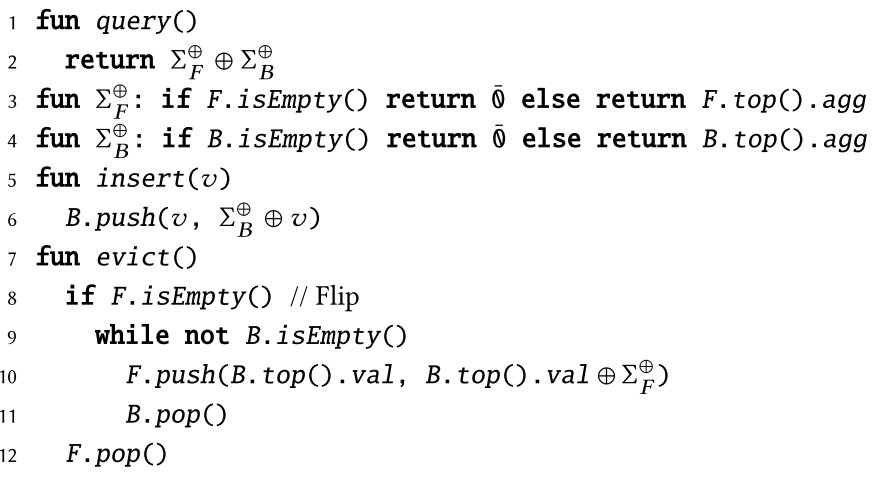
\includegraphics[scale=0.45]{figures/2-stacks.png}
      \caption{Two-Stacks algorithm}
      \label{fig:pseudo-2-stacks}
    \end{center}
\end{figure}

\subsubsection*{Time complexity analysis}
Querying the aggregation state of the window and inserting a new element can be performed in constant time. However, while evicting an item is usually done in constant time, occasionally, a flip operation is required, consuming \textit{O(n)} time, with \textit{n} as the size of stack B. Because this flip is occasionally performed, the time complexity of Two-Stacks is said to be \textit{amortized} constant.

\subsubsection*{Space complexity analysis}
Two-Stacks uses two stacks as auxiliary data structures. The combined size of both stacks is at most the size of the sliding window \textit{n}. Hence, Two-Stacks has linear space complexity \textit{O(n)}.

\subsubsection*{Applicability to our Hypothesis}
Two-Stacks is a general sliding window aggregation algorithm to compute \textit{associative} aggregations. However, it is linear in space and occasionally performs the computationally intensive operation of flipping stack B onto stack F, making it unfit for our use case.


\subsection{De-Amortized Banker’s Aggregator} \label{sec:daba}

The De-Amortized Banker’s Aggregator (DABA) \cite{Tangwongsan-DABA} is a SWAG algorithm that allows the computation of \textit{associative} aggregations. Quoting the authors: \textit{"Deamortization is a method that turns the average-case behavior into the worst-case behavior, usually by carefully spreading out expensive operations"}. Hence the name \textit{"De-Amortized"}, as the main idea behind DABA's design is to avoid occasional expensive operations --- such as the flip operation in Two-Stacks --- by gradually executing them throughout run time.

\subsection*{Data Structure}

DABA uses two queues, \textit{vals} and \textit{aggs}, both of size \textit{n}, seen in Figure \ref{fig:daba-ds}. Both queues share six pointers --- \textit{F, L, R, A, B} and \textit{E} --- that point to the same position for each queue. These pointers are always ordered as follows: $\textit{F} \leq \textit{L} \leq \textit{R} \leq \textit{A} \leq \textit{B} \leq \textit{E}.$

\begin{figure}[!htb]
    \begin{center}
      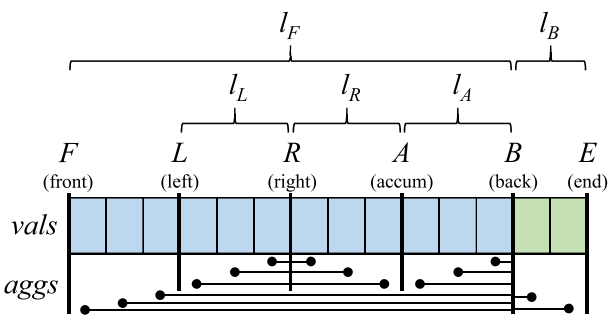
\includegraphics[scale=0.6]{figures/daba-ds.png}
      \caption{DABA data structure}
      \label{fig:daba-ds}
    \end{center}
\end{figure}

Queue \textit{vals} holds the actual sliding window contents. New values are pushed in the back and old values are popped from the front of the queue. Queue \textit{aggs} stores aggregations of sub-ranges of \textit{vals}. Aside from pointer \textit{E}, each pointer defines a sub-list and each sub-list is aggregated either to the left \textbullet--- or to the right ---\textbullet. If a sub-list is aggregated to the left \textbullet---, each \textit{aggs} element will be the aggregation value of all elements in \textit{vals} from that position to the right. On the other hand, if a sub-list is aggregated to the right ---\textbullet, each \textit{aggs} element will be the aggregation value of all elements in \textit{vals} from that position to the left. Values from \textit{vals} can be aggregated to the left or to the right because DABA restricts the aggregation to be \textit{associative} (refer to Table \ref{tbl:aggregations-properties}).

\textit{l\textsubscript{F}} is aggregated to the left for easier eviction. After an element is evicted, the new head of the queue \textit{aggs} --- pointed by \textit{F} --- already contains the aggregation value of all elements from \textit{vals} to its right side. Hence, evicting an element amounts to evicting from both \textit{vals} and \textit{aggs} queue. Similarly, \textit{l\textsubscript{B}} is aggregated to the right to facilitate insertion. Sub-lists \textit{l\textsubscript{L}}, \textit{l\textsubscript{R}} and \textit{l\textsubscript{A}} allow for incremental reversal of the right-aggregated \textit{l\textsubscript{B}} to the left-aggregated \textit{l\textsubscript{F}}. This incremental reversal is tantamount to adjusting pointers that causes shifts in sub-list boundaries. Thus, elements of \textit{aggs} may change from one sub-list to another and need to have its aggregation value recomputed.

Inserting a new element corresponds to pushing a new value \textit{val} in \textit{vals} and pushing the new aggregation value \textit{agg} in \textit{aggs}. The new aggregation value \textit{agg} is computed by applying the \textit{combine} function $\oplus$ to the back element of \textit{aggs} and the new value \textit{val} --- \textit{i.e.} pushing \textit{val} to \textit{vals} and $\textit{aggs[E]} \oplus \textit{val}$ to \textit{aggs}. 

Evicting old elements is done by evicting the same number of elements from \textit{vals} and \textit{aggs}.

\textit{l\textsubscript{F}} and \textit{l\textsubscript{B}} combined cover the whole \textit{vals} queue --- \textit{i.e.} every element in the sliding window. \textit{l\textsubscript{F}} is aggregated to the left, thus \textit{aggs[F]} contains the aggregation value of everything in \textit{l\textsubscript{F}}. On the other hand, \textit{l\textsubscript{B}} is aggregated to the right, thus \textit{aggs[E]} stores the aggregation value of everything in \textit{l\textsubscript{B}}. Hence, the aggregation value of the entire window will be the result of \textit{$aggs[F] \oplus aggs[E]$}.


\subsection*{Incremental Reversal of \textit{l\textsubscript{B}} to \textit{l\textsubscript{F}}}

The main conceptual difference between DABA and Two-Stacks is that in Two-Stacks an occasional expensive \textit{flip} operation takes place --- flipping stack B onto stack F --- and in DABA the reversal of \textit{l\textsubscript{B}} to \textit{l\textsubscript{F}} is incremental. This allows DABA to achieve constant time complexity (on average) rather than Two-Stacks' amortized constant time complexity.

Figure \ref{fig:pseudo-daba} shows the pseudocode presented by the authors for the DABA algorithm. In reality, after each insertion and eviction, besides the procedure already described, function \textit{fixup} is executed. The \textit{fixup} function performs the incremental reversal of \textit{l\textsubscript{B}} to \textit{l\textsubscript{F}}. The pseudocode \ref{fig:pseudo-daba} shows how such reversal is done but we will not elaborate on such procedure. However, it is important to stress out that this is the core idea of DABA: avoid occasional expensive operations, like Two-Stacks' \textit{flip}, by spreading them out across run time, in the form of DABA's \textit{fixup}.

\begin{figure}[!htb]
    \begin{center}
      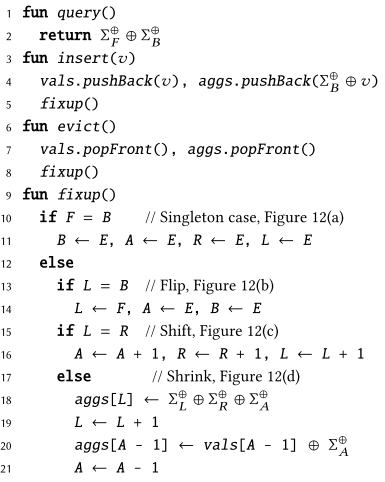
\includegraphics[scale=0.7]{figures/daba-pseudocode.png}
      \caption{DABA algorithm}
      \label{fig:pseudo-daba}
    \end{center}
\end{figure}


\subsection*{Time complexity analysis}
Querying the aggregation state as described is done in constant time. Insertion and eviction of elements take constant time and invoke function \textit{fixup}. The authors develop Theorems that prove function \textit{fixup} is executed in constant time as well. Hence, DABA has constant time complexity.

\subsection*{Space complexity analysis}
DABA stores the window contents in the \textit{vals} queue. Queue \textit{aggs} is of the same size as \textit{vals} and stores partial aggregations over \textit{vals}. Hence, if the window size is \textit{n}, DABA uses two \textit{n}-sized queues. Hence, DABA has \textit{O(n)} space complexity, meaning memory consumption grows linearly with window size.

\subsection*{Applicability to our Hypothesis}
Even though DABA improves on the time complexity of Two-Stacks, it still shows linear space complexity regarding window size. In our monitoring system, we need to analyze large windows of data, requiring at least logarithmic space complexity, thus making DABA inapplicable for our Hypothesis.


\textbf{TODO: Add table with SWAG algorithms, time and space complexity and applicable restrictions on the aggregation}

\section{Probabilistic Data Structures} \label{sec:pds}
In Section \ref{sec:sota-swag-algs} we presented some state-of-the-art algorithms for computing sliding window aggregations (SWAGs). However, if the aggregation we desire to compute can be approximated, there may exist more memory efficient methods. These aggregators are commonly denoted as sketches or probabilistic data structures and produce results orders-of magnitude faster then some exact approaches while keeping the memory consumption constant and providing mathematically proven error bounds. Each probabilistic data structure is used for efficient computation of one approximate aggregation, hence we say they are aggregation-specific.

Probabilistic data structures use hash functions to compactly represent a set of items. They require a single pass through the data, which is appropriate for a streaming scenario. Probabilistic data structures have constant space and time complexity \cite{Singh-PDS-BIGD} making them ideal aggregators to build our real-time and low memory footprint system. 

\subsection{Membership Queries and the Bloom filter} \label{sec:bloom}
% approx aggregation to compute
A Bloom filter \cite{BLOOM-BLOOMFILTER} approximate aggregator allows membership queries on a set of elements. Bloom filters answer the query: "Is element \textit{el} in the set of seen elements so far?". Being a probabilistic data structure and approximate aggregator, Bloom filters' answers have an error associated. \textit{False positive} matches are possible --- \textit{i.e.} saying \textit{el} is in the set when it is not --- but \textit{false negatives} are not --- \textit{i.e.} saying \textit{el} is not in the set but it actually is. In other words, a Bloom filter will accurately identify all items that do not belong in the set but will misclassify some items as being present in the set. Hence, a query returns either \textit{possibly in set} or \textit{definitely not in set}.

% data structures
\subsection*{Data structure}
A Bloom filter is an array of bits of size \textit{m}, initially all set to 0. Figure \ref{fig:initial-bloom-filter} represents a Bloom filter with a bit array of size \textit{m}=7 in its initial state.

\begin{figure}[!htb]
    \begin{center}
      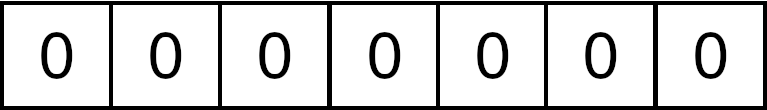
\includegraphics[scale=1.1]{figures/initial-bloom.png}
      \caption[Bloom filter initial state]{Bloom filter bit array initial state of \textit{m}=7}
      \label{fig:initial-bloom-filter}
    \end{center}
\end{figure}

% algorithm for insertion
\subsection*{Element Insertion}
Element insertion and query answering make use of \textit{k} hash functions, each mapping elements to a position in the bit array. Adding an element is done by determining which positions should be set to 1. To that end, the new element is fed into each hash function that maps the element to an array position. The resultant \textit{k} outputs are used as the \textit{k} positions of the array to be set to 1. Figure \ref{fig:insertion-bloom-filter} shows the insertion of element \textit{el} in the Bloom filter, making use of three hash functions (\textit{k}=3), \textit{h\textsubscript{1}}, \textit{h\textsubscript{2}} and \textit{h\textsubscript{3}}. The outputs of the hash functions correspond to the array indexes to set to 1.

\begin{figure}[!htb]
    \begin{center}
      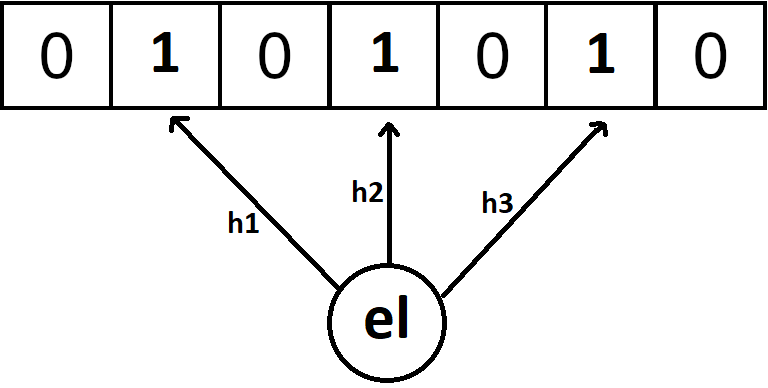
\includegraphics[scale=0.4]{figures/insert-bloom.png}
      \caption[Bloom filter insertion]{Insertion of element \textit{el} into a Bloom filter with \textit{m}=7 and \textit{k}=3}
      \label{fig:insertion-bloom-filter}
    \end{center}
\end{figure}

% algorithm for query
\subsection*{Membership Query}
Performing a membership query --- \textit{i.e.} testing if an element \textit{el} is in the set --- is done by feeding \textit{el} into each one of the \textit{k} hash functions in order to get an array of positions. If \textit{el} was already in the set, all \textit{k} positions should be 1. If any position contains a 0 then the element is \textit{definitely not in set}, as shown in Figure \ref{fig:bloom-filter}. 

\begin{figure}[!htb]
    \begin{center}
      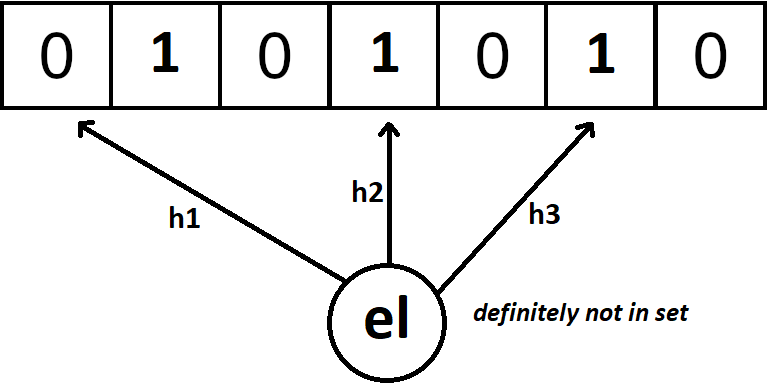
\includegraphics[scale=0.4]{figures/query-bloom.png}
      \caption[Bloom filter membership query]{Bloom filter membership test of element \textit{el}. Finding at least one '0' indicates that it is not in the set.}
      \label{fig:bloom-filter}
    \end{center}
\end{figure}

If all positions are 1 then the element is said to be \textit{possibly in the set}. The reason a Bloom filter does not provide 100\% certainty that \textit{el} is in the set in case of all positions being 1 is that hash functions may give the same position for two different elements. For example, hash functions \textit{h\textsubscript{1}}, \textit{h\textsubscript{2}} and \textit{h\textsubscript{3}} may map an element \textit{el1} to positions $[1,2,3]$ and an element \textit{el2} to positions $[4,5,6]$. This way, bits in positions $[1,2,3,4,5,6]$ are set to 1. When querying about the membership of a new element \textit{el3}, hash functions \textit{h\textsubscript{1}}, \textit{h\textsubscript{2}} and \textit{h\textsubscript{3}} may map it to positions $[1,3,5]$ as exemplified in Figure \ref{fig:bloom-filter-fp}. Since all of these positions are 1 because of the previous elements inserted, the Bloom filter returns \textit{"possibly in set"} when in reality \textit{el3} was not in the set. This is considered a \textit{false positive}.

\begin{figure}[!htb]
    \begin{center}
      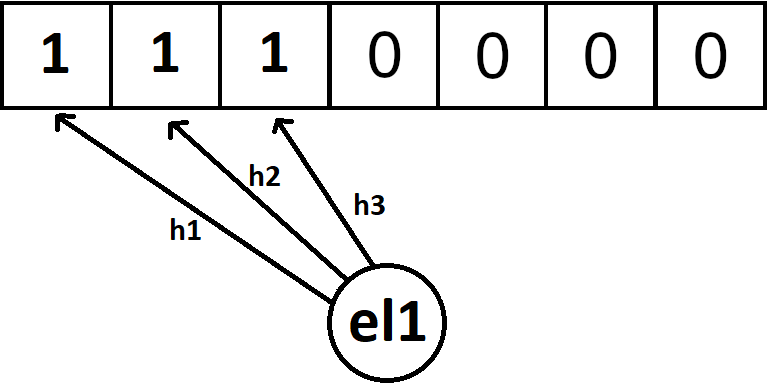
\includegraphics[scale=0.4]{figures/fp-bloom-1.png}
      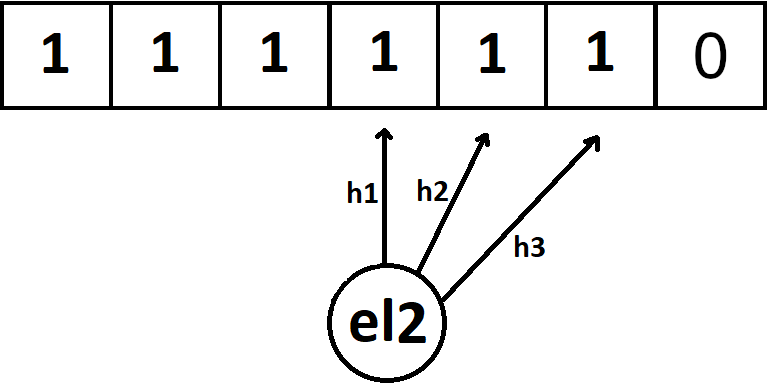
\includegraphics[scale=0.4]{figures/fp-bloom-2.png}
      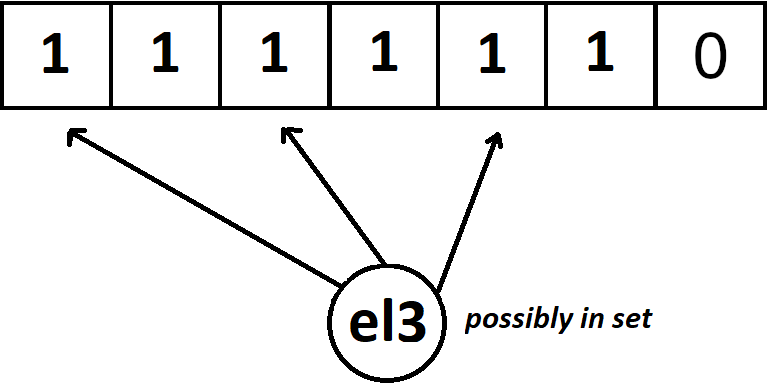
\includegraphics[scale=0.4]{figures/fp-bloom-3.png}
      \caption{Bloom filter false positive}
      \label{fig:bloom-filter-fp}
    \end{center}
\end{figure}


\subsection*{False Positive rate}
% error bound related with parameters
The false positive rate is a function of the bit array size \textit{m}, the number of hash functions \textit{k} and the number of elements in the set \textit{n}. It is assumed that the hash functions produce an independent and random index value for each element. Mullin presents an analysis of the Bloom filter in \cite{Mullin-Bloom-Analysis} where he details the false positive rate formula. 

The probability of one arbitrary bit being set to 1 is
\begin{equation}
    \frac{1}{m}
\end{equation}
because there are \textit{m} bits. Likewise, the probability of one bit not being set to 1 is
\begin{equation}
    1-\frac{1}{m}
\end{equation}

Mullin states the probability that an arbitrary bit is not set to 1 after one element insertion and corresponding \textit{k} bit updates is
\begin{equation}
    (1-\frac{1}{m})^\textit{k}
\end{equation}

For \textit{n} insertions, the probability a bit is not set to 1 is
\begin{equation}
    (1-\frac{1}{m})^\textit{kn}
\end{equation}

Therefore, the probability that an arbitrary bit is set to 1 after \textit{n} insertions is 
\begin{equation}
    1-(1-\frac{1}{m})^\textit{kn}
\end{equation}

Hence, the probability of false positive of a membership query for a new element for \textit{k} hash functions is given by
\begin{equation}
    (1-(1-\frac{1}{m})^\textit{kn})^\textit{k}
\end{equation}

This false positive rate can be approximated by 
\begin{equation}
    (1-e^\textit{-kn/m})^\textit{k}
\end{equation}


\subsection*{Optimal number of hash functions}
We want to choose the number of hash functions \textit{k} in order to minimize the false positive rate. In order to do so, we must first allocate \textit{m} bits for the Bloom filter, choosing \textit{m} based on available memory. The value of \textit{k} that minimizes the false positive rate is either of the nearest integers given by
\begin{equation}
    \frac{m}{n}ln(2)
\end{equation}

\subsection*{Time complexity analysis}
Considering a Bloom filter with \textit{m} bits and \textit{k} hash functions, insertion has \textit{O(k)} time complexity because all there is to do is run the input through all of the \textit{k} hash functions and set the bits in the given positions to 1. Similarly, query answering has \textit{O(k)} time complexity because it needs only to run the input through the \textit{k} hash functions and check if all bits are set to 1. If so, it returns \textit{possibly in set}. Otherwise it returns \textit{definitely not in set}. 

Note the time complexity does not at all depend on the number of elements in it and that \textit{k} will be a rather small constant. Hence, the Bloom filter is said to have constant time complexity.

\subsection*{Space complexity analysis}
Considering a Bloom filter with \textit{m} bits, the space required is simply the array of \textit{m} bits, thus \textit{O(m)} space complexity. Similarly to the time complexity analysis, we point out that \textit{m} will be constant and that each of the array elements occupies 1 bit. Thus the Bloom filter has a constant space complexity.

\subsection*{Applicability to our Hypothesis}
Bloom filters exhibit constant space and time complexity making it great methods to test our hypothesis. Their false positive rate is tolerable in most scenarios and can be controlled by tweaking the values of \textit{m} and \textit{k}.

\subsection{Item Frequency and the Count-Min Sketch}
% approx aggregation to compute
The Count-Min Sketch (CMS) uses two principles from the discussed Bloom filters in Section \ref{sec:bloom}. First, Bloom filters show that precision can be sacrificed to achieve space savings. Second, they are very similar at a technical level.

A Count–Min Sketch \cite{Cormode-CMS} is an approximate aggregator that estimates the frequency of each element in the data set. It is named after the two basic operations used to provide the estimate: counting (\textit{count}) and computing the minimum (\textit{min}).

% data structures
\subsection*{Data structure}
A CMS is represented by a two-dimensional array (or matrix) with width \textit{w} and depth \textit{d}. A CMS will make use of \textit{d} hash functions --- \textit{i.e.} each associated with one row of the matrix. Each hash function will map elements to a position between 1 and \textit{w} --- \textit{i.e.} the column of the two-dimensional array. Initially, all of the matrix positions are 0. Figure \ref{fig:initial-cms} represents the two-dimensional array used by the CMS and corresponding dimensions in its initial state. 

\begin{figure}[!htb]
    \begin{center}
      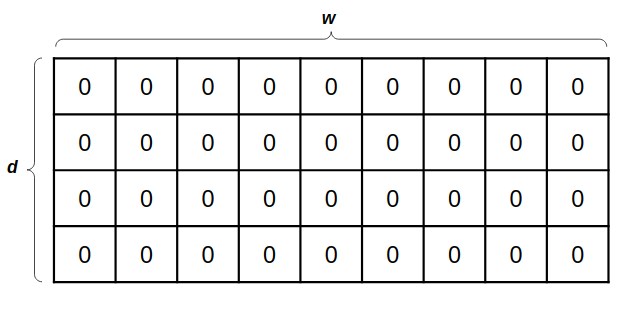
\includegraphics[scale=0.5]{figures/initial-cms.png}
      \caption[Count-Min Sketch initial state]{Count-Min Sketch matrix initial state of \textit{d}=4 and \textit{w}=9}
      \label{fig:initial-cms}
    \end{center}
\end{figure}

% algorithm for insertion
\subsection*{Element Insertion}
When adding an element, for each row \textit{i} of the \textit{d} rows in the matrix, hash the element using that row's hash function to obtain \textit{j}. Lastly, for all obtained pairs of \textit{i} and \textit{j}, increment matrix cells \textit{(i, j)} value by 1, as seen in Figure \ref{fig:cms}. If elements have different weights these can be added instead of incrementing one unit.

\begin{figure}[!htb]
    \begin{center}
      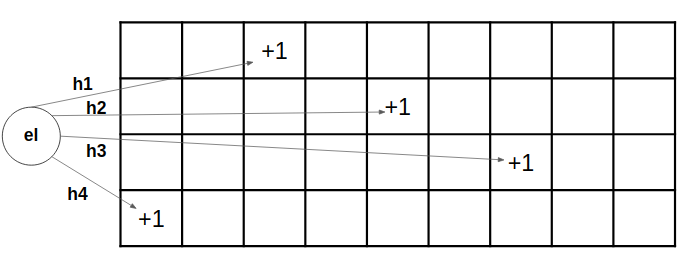
\includegraphics[scale=0.5]{figures/insertion-cms.png}
      \caption[Count-Min Sketch insertion]{CMS mapping element \textit{el} using \textit{d}=4 hash functions to determine the column position for each row and increment it}
      \label{fig:cms}
    \end{center}
\end{figure}

% algorithm for query
\subsection*{Frequency Query}
Retrieving the minimum frequency of an element \textit{el} can be done by taking the minimum value of all row counts for \textit{el}. Mathematically, the frequency estimate is the minimum value of the set of all row values, for each row \textit{i} of the total \textit{d} rows, given by
\[ min \{matrix[i][\textit{h\textsubscript{i}}(el)]\} \]

Figure \ref{fig:query-cms} illustrates this procedure, where the result of the query "What is the frequency of \textit{el}?" returns "2".
   
\begin{figure}[!htb]
    \begin{center}
      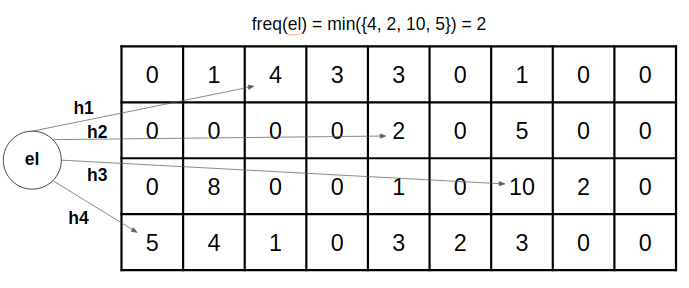
\includegraphics[scale=0.5]{figures/query-cms.png}
      \caption[Count-Min Sketch frequency query]{Count-Min Sketch frequency query of element \textit{el}}
      \label{fig:query-cms}
    \end{center}
\end{figure}

% error bound related with parameters
\subsection*{Optimal number of hash functions} 
For an element \textit{el}, each row will have one position incremented by \textit{el}'s true frequency. However, multiple elements may be mapped to the same position within a row, thus overlapping their frequencies. Hence, for an element \textit{el}, the CMS provides a frequency estimate that is greater or equal to the true frequency of \textit{el} in the set.

The number of hash functions \textit{d} to be used depends on the desired error probability. To achieve an error probability $\delta$, \textit{d} is given by the following expression:
\begin{equation}
    d = \lceil ln \frac{1}{\delta} \rceil
\end{equation}
For example, to achieve an error $\delta$ = 1\%, \textit{d} = 5 hash functions are necessary.

\subsection*{Time complexity analysis}
When adding an element, the Count-Min Sketch loops through each row and applies a constant in time hash function, updating the value of the target cell. Hence, insertion loops through \textit{d} rows and has time complexity of \textit{O(d)}. Similarly, querying the frequency of an element \textit{el} consists in computing the minimum of all row values. Since both insertion and query have constant time complexity, the CMS is constant in time.

\subsection*{Space complexity analysis}
The Count-Min Sketch relies on a two-dimensional matrix as its only data structure. The memory used will correspond to the \textit{wd} counts, hence \textit{O(wd)} space complexity. Since both \textit{w} and \textit{d} are constants, the CMS has constant space complexity.

\subsection*{Applicability to our Hypothesis}
Count-Min Sketches are constant in both time and space. Similarly to Bloom filters, this makes them ideal candidates for our solution. 

\subsection{Cardinality Estimation and the HyperLogLog} \label{sec:hyper-log-log}

A set of probabilistic counting algorithms is introduced by Flajolet et al. in \cite{Flajolet-PCA} to estimate the number of distinct elements of a set --- also known as the cardinality of the set. These techniques are based on \textit{"bit-pattern observables"} in the binary representation of the hashed values. Bit-pattern observables are defined by the authors as \textit{"patterns of bits occurring at the beginning of the (binary) S-values"}, with \textit{S} as the target set.

Later on, the authors propose the LogLog algorithm \cite{Flajolet-LogLog}. In LogLog, the bit-pattern observable recorded for each item is the position of the leftmost 1-bit, denoted as \textit{P}. The authors claim it is related to the total number of distinct elements in the data set in that it is \textit{"more or less a likely indication that the cardinality of S is at least $2^P$"}.


% FOR EACH SKETCH DO:
% approx aggregation to compute
% data structures
% algorithm for insertion
% algorithm for query
% error bound related with parameters
% time complexity analysis
% space complexity analysis
% Applicability to our Hypothesis
\subsection*{HyperLogLog}
A couple of years later, the same authors propose HyperLogLog (HLL) \cite{Flajolet-HLL}, an approximate aggregator to compute the cardinality of a set. 

HLL uses the same bit-pattern observable as LogLog --- \textit{P}, the position of the leftmost 1-bit. With LogLog, the authors realize that storing only one observation produces extremely inaccurate predictions due to the high variability of a single value. The proposed solution is to apply \textit{stochastic averaging}. As the authors state, stochastic averaging \textit{"consists in emulating the effect of m experiments"}. Effectively speaking, the authors propose dividing the input stream into \textit{m} substreams or buckets, maintaining one observable per bucket and computing \textit{P} as an average of all bucket values (stochastic averaging).

\subsection*{Data Structure}
HyperLogLog (HLL) maintains \textit{m} bit-pattern observables, each being the leftmost 1-bit position, \textit{P}. Since each position is a single integer, HLL maintains \textit{m} integer counters, as seen in Figure \ref{fig:hll-ds}. Each of these counters holds the maximum value for the bit-pattern observable seen so far. The first bit is assumed to be in position "1" and all counters begin with "0".

\begin{figure}[!htb]
    \begin{center}
      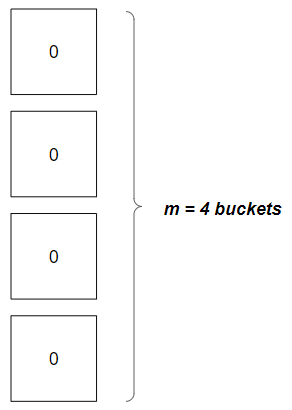
\includegraphics[scale=0.6]{figures/hll-ds.png}
      \caption[HyperLogLog initial state]{HyperLogLog with \textit{m}=4 observable buckets}
      \label{fig:hll-ds}
    \end{center}
\end{figure}


\subsection*{Element Insertion}
In HyperLogLog, new elements are hashed into a binary string. The first \textit{n} bits of the hashed representation will map to one of the \textit{m}=$2^n$ buckets. Effectively speaking, the first \textit{n} bits work as a \textit{bucket ID}. The bit-pattern observable \textit{P} --- the position of the leftmost 1-bit --- is counted from the binary string discarding the first \textit{n} bits. The observable \textit{P} is stored in the pre-determined bucket if it is greater than the value the bucket contains. 

Figure \ref{fig:hll-insert} demonstrates such procedure for a new element \textit{el}. The hash representation of \textit{el}, using \textit{n}=2 bits, maps to bucket \textit{10}. Discarding the first \textit{n}=2 bits and counting from 1, the position of the leftmost 1-bit is \textit{P}=4. The previous value of bucket \textit{10} was 0 and because \textit{P}=4 is greater than 0 the bucket value is updated.


\begin{figure}[!htb]
    \begin{center}
      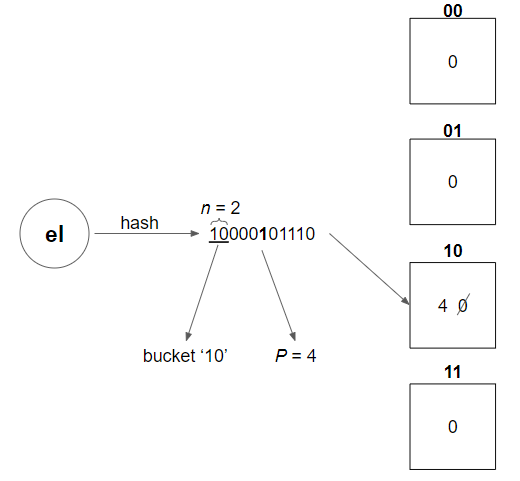
\includegraphics[scale=1]{figures/hll-insertion.png}
      \caption[HyperLogLog insertion]{HyperLogLog \textit{el} insertion with \textit{m}=4 and \textit{n}=2 bits}
      \label{fig:hll-insert}
    \end{center}
\end{figure}

\subsection*{Cardinality Query}
The cardinality of the set is estimated to be $2^\textit{P}$ where the bit-pattern observable \textit{P} is the position of the leftmost 1-bit. As discussed, HyperLogLog (HLL) differentiates from LogLog in that it applies a stochastic averaging process. Hence, the value of \textit{P} will be the harmonic mean of all \textit{m} buckets.


\subsection*{Time complexity analysis}
Adding an item is tantamount to hashing it, determining the corresponding bucket based on the first \textit{n} bits, counting the leftmost 1-bit position and updating the bucket value if need be. Estimating the cardinality of the set amounts to finding the maximum value \textit{P} between all buckets and computing $2^P$. Hence, both inserting a new element and estimating the cardinality of the set take constant time.

\subsection*{Space complexity analysis}
Quoting Flajolet et al. about the memory consumption and error in the approximations obtained in their experiments in the original HyperLogLog paper \cite{Flajolet-HLL}: 
\say{cardinalities till values over N = $10^9$ can be estimated with a typical accuracy of 2\% using 1.5kB (kilobyte) of storage.}

HyperLogLog uses \textit{m} buckets that store a single integer value, thus the space complexity is \textit{O(m)} where \textit{m} is a rather small constant. Hence, HyperLogLog has constant space complexity.

\subsection*{Applicability to our Hypothesis}
Similar to the previously studied approximate aggregators, HyperLogLog (HLL) has constant space and time complexity and provides an estimate of a set's cardinality. Hence, HLLs are considered valuable aggregators for our Thesis.

\iffalse
%TODO: Worth to show? HLL uses only one hash, only CMS and Bloom benefit from this.
\subsection{Hash improvement}
An improvement to this structure was defined in \cite{Kirsch-Better-Bloom} where the authors attempt to reduce the overhead of bloom filters operations such as adding a new element or answering a query by focusing on the hash functions. The proposed method is based on hashing literature. It has been shown that multiple hash functions can be created from the combination of only two hash functions. This means that a new hash function \textit{g} can be produced based on  two other independent and uniform existing hash functions, \textit{h1} and \textit{h2}. The new hash function will map elements to a universe ranging from \textit{0} to \textit{p-1} and will be defined as \textit{$g(x) = h1(x) + ih2(x) mod p$}. Since the only nontrivial computations performed by a Bloom filter are the evaluations of pseudo-random hash functions, any reduction in the required number of pseudo-random hash functions yields a reduction in the time required to add an element or query a Bloom filter.

Bloom filters are not the only approximate aggregators that use hash functions as a basis of their algorithm. All of the studied probabilistic data structures do so. Therefore, the technique proposed is beneficial in Count-Min Sketches and Bloom filters.
\fi

\section{Sliding Window Aggregations with Probabilistic Data Structures}
In Section \ref{sec:pds} we presented a set of probabilistic data structures constant in time and space. These structures aggregate an endless stream of data. However, when working with sliding windows there is the need not only to insert new events but to evict old ones. Probabilistic data structures aggregate all incoming data but have no way of expiring old elements from the aggregation state. 

The probabilistic data structures studied can be implemented under generic sliding window aggregation algorithms like Recalculate-From-Scratch or DABA. However, doing so means we lose the main advantage of using these approximate aggregators: the constant space complexity. For example, cardinality estimation of a sliding window can be done employing the HyperLogLog heuristic of estimating cardinality as $2^\textit{p}$, with \textit{p} as the maximum position seen for the leftmost 1-bit, using DABA \ref{sec:daba} for the computation of \textit{p} per sliding window. With this approach, despite computing the aggregation state in constant time, we have a linear in window size space complexity solution. Thus, in this Section, we explore sliding window implementations of the previously discussed probabilistic data structures that keep the space and time complexity at the very least logarithmic.

%\subsection{Sliding Bloom filter}
%\subsection*{Data Structure}
%\subsection*{Element Insertion}
%\subsection*{Element Eviction}
%\subsection*{Time complexity analysis}
%\subsection*{Space complexity analysis}
%\subsection*{Applicability to our Hypothesis}

%\subsection{Sliding Count-Min Sketch}
%\subsection*{Data Structure}
%\subsection*{Element Insertion}
%\subsection*{Element Eviction}
%\subsection*{Time complexity analysis}
%\subsection*{Space complexity analysis}
%\subsection*{Applicability to our Hypothesis}


\subsection{Sliding HyperLogLog}

The HyperLogLog (HLL) aggregator presented in Section \ref{sec:hyper-log-log} will only be useful to us if it can be implemented efficiently in a sliding window fashion. The HLL aggregator estimates the set's cardinality assuming it is close to $2^\textit{p}$, where \textit{p} is the maximum position seen for the leftmost 1-bit in the binary values of all of the set items' hashes. In practice, all the aggregator has to compute is \textit{p}, the maximum value of all observables. Stochastic averaging is applied by emulating the effects of \textit{m} experiments using \textit{m} buckets to store \textit{m} bit-pattern observables. 


\subsubsection{Sliding HyperLogLog using Lists of Future Possible Maxima} \label{sec:hll-lfpm}

The work of Chabchoub et al. adapts the original HLL aggregator from Flajolet et al. to work under a sliding window framework  \cite{Chabchoub-Sliding-HLL}.
The main idea behind this implementation is to replace every HLL counter with a \textit{"List of Future Possible Maxima (LFPM)"}.

\subsubsection*{Data Structure}

The adaptation of the original HLL to work under a sliding window scenario requires the storage of additional information. The original HLL maintained \textit{m} integer counters, each storing the maximum for the leftmost 1-bit position of the analyzed binary strings.  The counter held the maximum value for all the seen binary strings so far but there was no way to expire old items. To allow eviction, the proposed data structure is very similar to the original \textit{m} integer counters but keeps a list of values per bucket and associates a timestamp to each. 

The stochastic averaging process of HLL remains unchanged: incoming items are hashed and distributed across \textit{m} buckets. However, the authors propose keeping a short list of \textit{packets} per bucket instead of a single integer count. A \textit{packet} is defined as a pair <\textit{t\textsubscript{i}, p\textsubscript{i}}> where \textit{t\textsubscript{i}} is the arrival timestamp of the packet and \textit{p\textsubscript{i}} the position of the leftmost 1-bit in the binary hash representation of the associated value. Packets are only kept in the list if they are possible maxima over future windows. Because of that, the authors name this list a \textit{"List of Future Possible Maxima (LFPM)"}.

\subsubsection*{Element Insertion \& Eviction}
Similarly to the original HLL, incoming elements are hashed and the first \textit{n} bits of the string are used to map the new element to one of the \textit{m} buckets. The first \textit{n} bits are then discarded and the bit-pattern observable \textit{p} is computed from the remaining string. 

Since each bucket now holds a LFPM instead of a single integer, the procedure for bucket update is different. Upon insertion of an element \textit{k}, a packet <t\textsubscript{k}, p\textsubscript{k}> is created with t\textsubscript{k} as the timestamp of arrival of the new element \textit{k} and p\textsubscript{k} as the position of the leftmost 1-bit position of \textit{k}'s binary representation. Given the new packet <t\textsubscript{k}, p\textsubscript{k}>, the authors propose the following LFPM update method, that checks for and evicts old packets at each insertion:

\begin{itemize}
    \item Delete \textit{old packets}: packets that do not belong in the window anymore --- \textit{i.e.} packets <t\textsubscript{i}, p\textsubscript{i}> with t\textsubscript{i} $\leq$ t\textsubscript{k} - WindowSize 
    
    \item Delete less or equally valued packets: packets that will never be a maximum --- \textit{i.e.} packets <t\textsubscript{i}, p\textsubscript{i}> with p\textsubscript{i} $\leq$ p\textsubscript{k}
    
    \item Add the new packet <t\textsubscript{k}, p\textsubscript{k}>
\end{itemize}


\subsubsection*{Sliding Window Cardinality Query} 

Estimation of cardinality is done similarly to the original HLL cardinality estimation algorithm. To estimate the cardinality at a timestamp \textit{t}, from all \textit{m} buckets and all \textit{m} lists, select packets that are in the window --- \textit{i.e.} packets <t\textsubscript{i}, p\textsubscript{i}> where t\textsubscript{i} > \textit{t} - WindowSize. This filtering is necessary since the proposed algorithm evicts old packets only at element insertion and at the time of the query some packets may no longer belong to the window. Next, from the filtered set of packets, for each bucket and its list, compute the maximum p\textsubscript{i} value. In the end, compute the harmonic mean between all values, just like the original HLL. The result will be the averaged bit-pattern observable value \textit{p} and the cardinality is estimated to be $2^\textit{p}$.

\subsubsection*{Time complexity analysis}
When performing insertions or evictions, the algorithm requires scanning through the Lists of Future Possible Maxima (LFPMs) to delete old packets or packets that will never be window maxima. Similarly, we need to scan the lists when estimating the cardinality to filter for packets within our window. Denote \textit{L\textsubscript{n}} as the mean size in packets for each LFPM. There are \textit{m} buckets, each with a list. To scan through all lists we need to analyze \textit{m L\textsubscript{n}} elements. 

The authors prove that \textit{L\textsubscript{n}} has an upper bound of \textit{ln(n/m)}, with \textit{n} as the cardinality of the set and \textit{m} as the number of buckets used. Hence, in the worst-case scenario, we need to analyze \textit{m ln(n/m)} elements. This means that a Sliding HLL implementation using Lists of Future Possible Maxima has \textit{O(ln(n))} time complexity, given the number of buckets \textit{m} is constant.

\subsubsection*{Space complexity analysis}
The memory used in the Sliding HLL aggregator implemented with Lists of Future Possible Maxima (LFPMs) amounts to the total size of the \textit{m} lists. Assuming 4 byte timestamps and 1 byte bit-pattern observables for each packet, the aggregator uses \textit{(4+1) L\textsubscript{n} m} bytes. 

The lists are dynamic thus they shrink and grow at run time. However, \textit{ln(n/m)} was proved to be an upper bound for \textit{L\textsubscript{n}}. Hence, this sliding implementation of the HLL aggregator consumes up to \textit{(4+1) ln(n/m) m} bytes of memory. Considering that the number of buckets \textit{m} is constant, the space complexity of a Sliding HLL implementation with LFPM is \textit{O(ln(n))}.

The authors claim that the proposed sliding version remains as accurate as the original HLL aggregator. In the context of their work, each element in the set is denoted as a "flow" and they state that \textit{"In practice, with an additional memory of only 35kB, a standard error of about 3\% can be achieved for a data stream of several million flows"}.


\subsubsection*{Applicability to our Hypothesis}
Implementing a Sliding HLL using Lists of Future Possible Maxima (LFPMs) shows logarithmic time and space complexity while providing estimates with the same accuracy as the original HLL approximate aggregator. However, the memory consumption is dynamic due to the variable size of the lists. 

Despite the fact memory consumption dynamically changes during runtime, this is a valid approach to test our Hypothesis due to the worst-case scenario being a logarithmic space complexity. However, in Section \ref{sec:hll-drv} we analyze an implementation that is not dynamic in memory during run time making it a preferred approach.


\subsubsection{Sliding HyperLogLog using Distance Recorder Vectors} \label{sec:hll-drv}

In Section \ref{sec:hll-lfpm} we have analyzed a Sliding HLL implementation where each of the \textit{m} buckets holds a list of values (LFPM) instead of a single integer count. However, the LFPM structure is dynamic and its size varies at run time. 

The approach proposed by Xu uses a smaller amount of memory that does not change at run time \cite{Xu-hll-sliding-drv}. The author proposes a special counter: a \textit{"Distance Recorder Vector (DRV)"}. 

\subsubsection*{Data Structure}
Much like the original HLL and the LFPM Sliding implementation, the Distance Recorder Vector (DRV) approach uses \textit{m} buckets. However, instead of integer counts or lists, each of the buckets stores a DRV. 

A DRV is composed by \textit{$\lceil ln(n/m) \rceil$} records, with \textit{n} as the cardinality of the set. Notice that \textit{n/m} is the average number of distinct elements each bucket \textit{m} is expected to process and that a binary string of size \textit{$\lceil ln(n/m) \rceil$} can represent \textit{n/m} distinct elements. Also recall that the bit-pattern observable \textit{p} used by the HLL is the position of the leftmost 1-bit. In a binary string of size \textit{$\lceil ln(n/m) \rceil$}, \textit{p} will range from 1 to \textit{$\lceil ln(n/m) \rceil$}. The DRV is indexed exactly this way, from 1 to \textit{$\lceil ln(n/m) \rceil$}, and each bit-pattern observable \textit{p} will be used as an index in this vector of records. Essentially, each \textit{p} will have an associated record in a DRV of a bucket.

Initially, all records in the DRV will be set to be infinity or a large number.

\subsubsection*{Element Insertion}
When an element is inserted, the same procedure as in the original HLL is followed: the element is hashed and \textit{p} is computed from the hashed binary representation. Denote the bit-pattern observable of the new element as \textit{p\textsubscript{new}}. For the DRV of that bucket, increment the value of all records by one. Next, set position \textit{p\textsubscript{new}} in the DRV to 0 (DRV[\textit{p\textsubscript{new}}] = 0).


\subsubsection*{Sliding Window Cardinality Query} 
Element eviction is not performed. Instead, the query algorithm takes into account that some records in some of the DVR's might not be valid anymore. To estimate the sliding window cardinality is to find the value \textit{p}. 

To find the value \textit{p} for a bucket, scan the DRV of that bucket backward. Start at the last element --- positioned at \textit{$\lceil ln(n/m) \rceil$} --- and scan towards the head of the vector. For each record, check if it is active in the current window. To do so, check if its value is less than the size of the window. If it is, the record is active. Otherwise, the record is inactive.

If the record is inactive continue scanning backward. If the record is active, then the position or index currently being scanned is the value of \textit{p} for that bucket. If all records are inactive, the bit-pattern observable \textit{p} is 0.

Stochastic averaging is done just like in the original HLL: compute the harmonic mean of all \textit{p\textsubscript{m}} values from all \textit{m} buckets. The cardinality of the sliding window is then estimated to be $2^\textit{p}$.

\subsubsection*{Time complexity analysis}
When inserting an element, determining its bucket, hashing the element and computing \textit{p} is done in constant time. However, all the  \textit{$\lceil ln(n/m) \rceil$} records must have their value increased by one and this means iterating over the DRV. Setting the element of the DRV indexed by \textit{p} to 0 is done in constant time as well. 

Estimating cardinality is done by scanning the DRV backward until an active record is found. In the worst-case scenario, this means scanning all \textit{$\lceil ln(n/m) \rceil$} records.

Both inserting an element and estimating sliding window cardinality require a scan through \textit{$\lceil ln(n/m) \rceil$} records. This gives us a time complexity of \textit{O(\textit{ln(n)})}, given the number of buckets \textit{m} is constant. 

\subsubsection*{Space complexity analysis}
This approach still uses \textit{m} buckets but each one contains a Distance Recorder Vector (DRV). A DRV is a vector of \textit{$\lceil ln(n/m) \rceil$} elements. Hence, \textit{$m \lceil ln(n/m) \rceil$} elements must be kept in memory, giving us a space complexity of \textit{O(ln(n))} with \textit{n} as the cardinality of the set.

\subsubsection*{Applicability to our Hypothesis}
Despite having the same time and space complexities, the Sliding HLL DRV approach uses a smaller amount of memory that does not change during runtime, while the LFPM requires heap resizing because the lists dynamically shrink and grow. Hence, the DRV approach is a better fit to integrate our lightweight real-time solution.




